\documentclass[]{scrartcl}
\usepackage{graphicx}
\usepackage{amsmath} % For equation alignment, bmatrix
\usepackage{amssymb} % For special math characters such as E with two vertical lines (expectation value symbol), Real numbers symbol, etc
\usepackage{witharrows} % For an aligned math environment where arrows show which transformation steps were taken
%\usepackage{mathtools} % For some extra math-related functionality, such as matrix*
%\usepackage{hyperref} % For using \autoref
%\usepackage{listings} % For adding code to the latex document
\usepackage{caption} % For adding captions
\usepackage{subcaption} % For adding subfigures and subcaptions
\usepackage{hyperref} % For referencing plots, tables, etc.
\usepackage{color} % For color in code
%\usepackage{nicematrix} % For creating matrices with outer rows and columns, with dsahed line separators. Documentation: https://ctan.org/pkg/nicematrix
\usepackage{float} % For better control over float environments
%\usepackage[utf8]{inputenc} % this is needed for umlauts
%\usepackage[ngerman]{babel} % this is needed for umlauts
%\usepackage[T1]{fontenc}    % this is needed for correct output of umlauts in pdf




% Opening / Title
\title{Complex Systems in Bioinformatics \\ \vspace{2mm} Exercise 7 \\ \vspace{2mm}}
\subtitle{Lecturers: Prof. Dr. Max von Kleist, Prof. Dr. Jana Wolf, Prof. Dr. Martin Vingron}
\author{Kristian Reinhart, 4474140 \\ Duong Ha Le Minh, 5314209}
\newenvironment{tightcenter}{%
  \setlength\topsep{0pt}
  \setlength\parskip{0pt}
  \begin{center}
}{%
  \end{center}
}




%%%%%%%%%%%%%%%%%%%%%%%%%%%%%%%%%%%
%%%	Begin actual document	%%%
%%%%%%%%%%%%%%%%%%%%%%%%%%%%%%%%%%%


\begin{document}

\maketitle


\section*{7. Assignment}

%%%%%%%%%%%%%%%%%%%%%%%%%%%%%%%%%%%
%%%			Exercise ODE		%%%
%%%%%%%%%%%%%%%%%%%%%%%%%%%%%%%%%%%

\subsection*{ODE System}

\textit{Quad-well potential:
\begin{center}
\begin{align*}
	V(z) & = (\vert z_1 \vert - 1)^2 + (\vert z_2 \vert - 1)^2
\end{align*}
\end{center}
}



%%%%%%%%%%%%%%%%%%%
%%%	Homework 1)	%%%
%%%%%%%%%%%%%%%%%%%

\subsubsection*{Homework 1}

The ODEs (from what I understood):
$$
\frac{dz_1}{dt} = -\frac{\partial V}{\partial z_1}
$$

$$
\frac{dz_2}{dt} = -\frac{\partial V}{\partial z_2}
$$

$$
\frac{\partial V}{\partial z_1} = \frac{\partial}{\partial z_1} \left[ (|z_1|-1)^2 + (|z_2|-1)^2 \right] = \frac{\partial}{\partial z_1} \left( (|z_1|-1)^2 \right) = 2(|z_1|-1) \cdot \frac{\partial}{\partial z_1}(|z_1|-1)
$$

$$
\frac{\partial}{\partial z_1} |z_1| = \text{sgn}(z_1)
$$

$$
\frac{\partial V}{\partial z_1} = 2(|z_1|-1) \cdot \text{sgn}(z_1)
$$

For the $z_1$ direction:
$$
\frac{dz_1}{dt} = - \frac{\partial V}{\partial z_1} = -2(|z_1|-1) \cdot \text{sgn}(z_1)
$$
Since $\text{sgn}(z_1) \cdot |z_1| = z_1$:
$$
\frac{dz_1}{dt} = 2(1-|z_1|) \cdot \text{sgn}(z_1) = 2(\text{sgn}(z_1) - |z_1|\text{sgn}(z_1)) = 2(\text{sgn}(z_1) - z_1)
$$
Analogous for the $z_2$ direction:
$$
\frac{dz_2}{dt} = - \frac{\partial V}{\partial z_2} = 2(\text{sgn}(z_2) - z_2)
$$


%%%%%%%%%%%%%%%%%%%
%%%	Homework 3)	%%%
%%%%%%%%%%%%%%%%%%%

\subsubsection*{Homework 3b)}

\begin{figure}[h!]
    \centering
    \begin{subfigure}[c]{0.49\textwidth}
        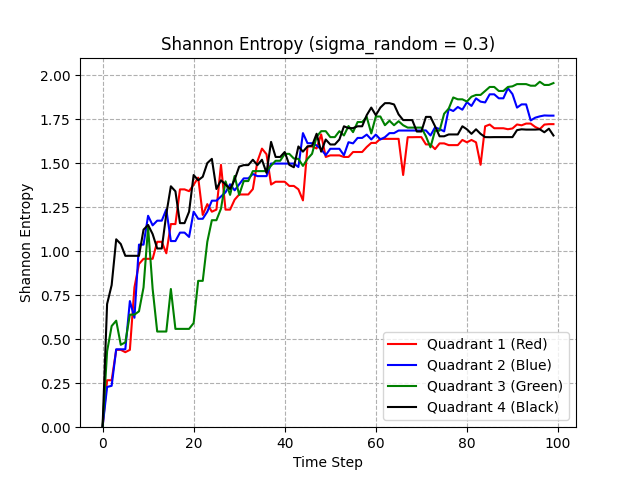
\includegraphics[width=\linewidth]{Shannon_Entropy_(sigma_random_=_0.3).png}
        %\caption{Subplot caption}
    \end{subfigure}\hfill
    \begin{subfigure}[c]{0.49\textwidth}
        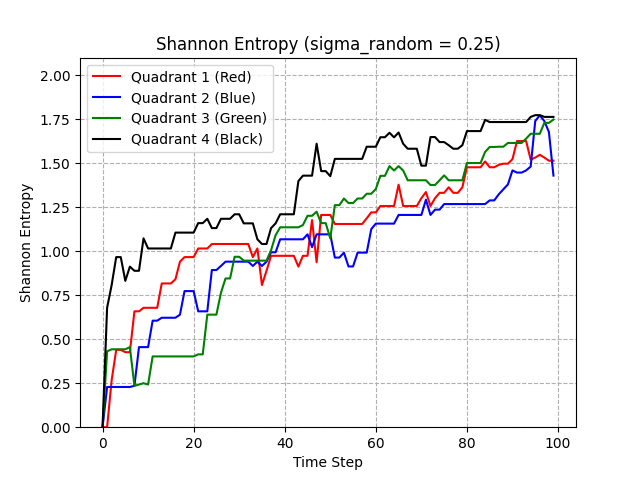
\includegraphics[width=\linewidth]{Shannon_Entropy_(sigma_random_=_0.25).png}
        %\caption{Subplot caption}
    \end{subfigure}\hfill
    \begin{subfigure}[c]{0.49\textwidth}
        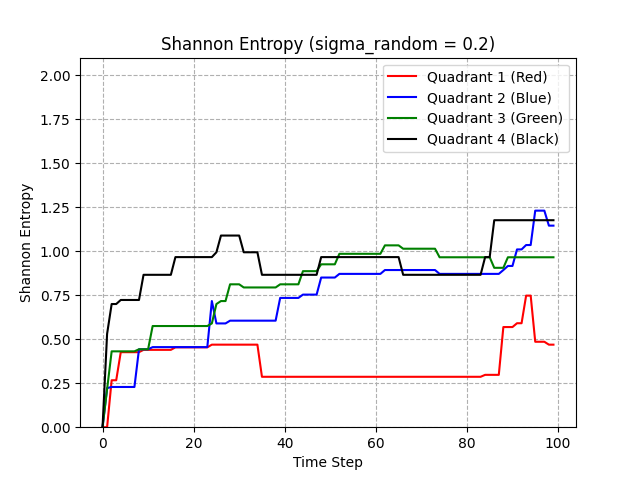
\includegraphics[width=\linewidth]{Shannon_Entropy_(sigma_random_=_0.2).png}
        %\caption{Subplot caption}
    \end{subfigure}\hfill
    \begin{subfigure}[c]{0.49\textwidth}
        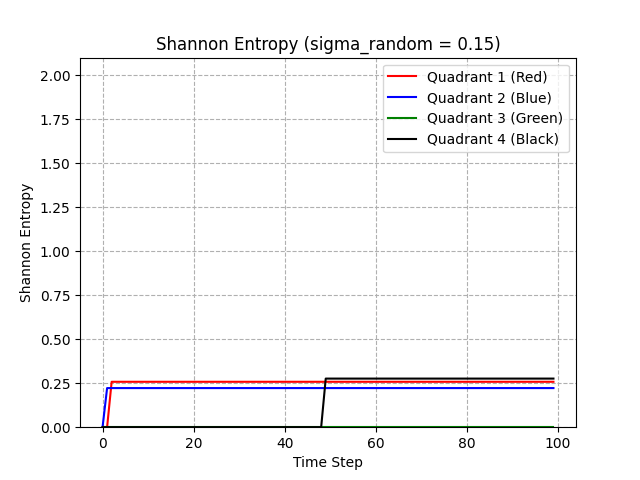
\includegraphics[width=\linewidth]{Shannon_Entropy_(sigma_random_=_0.15).png}
        %\caption{Subplot caption}
    \end{subfigure}\hfill
    \begin{subfigure}[c]{0.49\textwidth}
        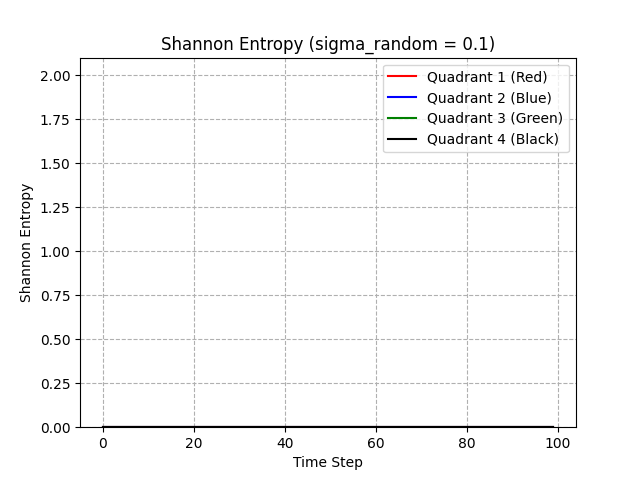
\includegraphics[width=\linewidth]{Shannon_Entropy_(sigma_random_=_0.1).png}
        %\caption{Subplot caption}
    \end{subfigure}
    \caption{Figures showing a reduction in entropy with a reduction of the random noise term $\sigma_{random}$ due to the simulated particles becoming trapped in the potential wells.}
    \label{fig:ShannonEntropy}
\end{figure}

In the particle-based diffusion model the potential is scaled by the drift weight $\sigma_{drift}$. Intuitively for the given quad-well potential this term scales how deep the wells are and represents a likelihood or preference for particles to stay in the region of the wells.
\\
The random noise factor $\sigma_{random}$ on the other hand is a factor for scaling the random motion of the simulated particles. A higher factor allows for larger movements per time step.
\\ \\
In the given task the drift weight $\sigma_{drift}$ stayed constant while the random noise factor $\sigma_{random}$ was consecutively reduced. The impact of the reduction can be observed in \autoref{fig:ShannonEntropy}. The gradual reduction of the entropy can be observed with a decrease in random movement due to the reduction of the noise $\sigma_{random}$ until finally somewhere between $\sigma_{random}=0.15$ and $\sigma_{random}=0.1$ the andom movement of the particles is unable to overcome the potential. Therefore the particles remain trapped in their respective wells of each quadrant and no mixing between the four different types takes place anymore.


\end{document}




